\section{Methodology}
\label{sec:methodology}
% Focus on what you add to the existing method. Explain what you will do and why (and how). Do not forget to characterize your research design. There should be a sub-section on the evaluation. 
%For DS students, this normally means using manually labelled or ground truth data. For IS students, it is not always needed to have a separate methodology section. You can also integrate the approach with the results in one section. It depends on your type of research what is best fitting.
\subsection{Data}
\label{data}
To investigate the impact of anonymization techniques on the accuracy of machine learning models, we used two real data sets: Early stage diabetes risk prediction\cite{ucidiabetes} and adult\cite{UCIAdultDataset}, which are both publicly available on the UCI Machine Learning Repository. The data set in question has been widely used to evaluate binary classifiers and privacy preserving techniques as they contains demographic information about individuals\cite{rodriguez2020contribution,oprescu2022energy}. These dataset is a common benchmark for evaluating machine learning models in the area of privacy-preserving data analysis\todo{ref}. For the details about the data referee to appendix \ref{Early Stage Diabetes}.\\
The use of early stage diabetes data for privacy-enhancing techniques depends on various factors, including the nature and sensitivity of the data, the privacy risks involved, and the specific technique being used.\todo{ref}In general, medical datasets, including early stage diabetes data, are considered to be highly sensitive due to the personal and sensitive nature of the information they contain. As such, they require strong privacy protections to ensure that individuals' privacy is not compromised. Privacy-enhancing techniques, such as differential privacy, k-anonymity, and secure multi-party computation, can be used to protect the privacy of individuals in medical datasets while still allowing useful analysis to be performed on the data.\todo{ref}.\\
The adult data set, which is also known as the Census Income dataset, taken in 1994 has 48,842 instances with 14 attributes and a labeled target attribute, salary. it includes attributes such as age, education level, occupation, marital status, and income. The goal of the dataset is to predict whether an individual's income is greater than or equal to 50,000 per year based on their demographic information\ todo{ref}. \\
First classify the data using ML algorithm on the original data set, un-anonymized data\ref{fig:Machine Learning Process And Scenarios} and then the same algorithms are applied to the identical(the same) data after it has been anonymized using the privacy framework \ref{fig:anonymization}. This approach is useful in cases where it is necessary to protect the privacy of individuals in the data, but also important to maintain the utility of the data for analysis or other purposes\cite{wimmer2014comparison}.\\
\subsubsection{Data Pre-Processing}
Data pre-processing is a technique used to convert raw data into a clean or ready dataset \cite{han2012}. The data pre-processing phase is crucial in the learning process of the algorithm, because different algorithms require different data pre-processing \cite{han2012}.  
\subsubsection{Initial data exploration and cleaning}
\begin{itemize}
    \item Early stage diabetes risk prediction: This dataset comprises 520 records which were collected using direct questionnaires from the patients of Sylhet Diabetes Hospital in Sylhet, Bangladesh in the year 2020. It contains binary and real features related to medical conditions and characteristics of patients admitted to the Sylhet Diabetes Hospital. It is a balanced dataset with 16 features in total including the age and gender of the participants. The data we consider as private attributes for our analysis is only the age though.\todo{ref}.
\end{itemize}
\subsubsection{Data anonymization and Data transformation}
\begin{itemize}
    \item k-anonymity: The first step in implementing was to identify the attributes as identifier, non-identifier and quasi-identifier (somewhat identifying) \todo{ref}. The attributes we use as quasi-identifiers are age, education, marital-status, sex, capital-gain, and hours-per-week of the Adult dataset while ..... are identied as a quasi-identifiers in Early stage diabetes risk prediction.
    \item Differential Privacy:
\end{itemize}
\subsection{Framework(setup) Experiment}
\begin{figure}[htb!]
    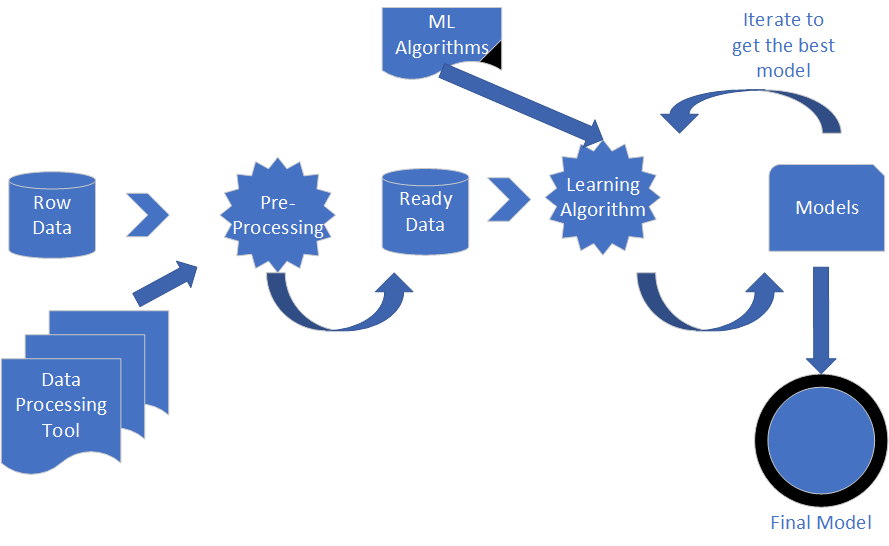
\includegraphics[scale=0.325]{media/framework/ml process.png}
    \caption{Machine Learning Process And Scenarios}
    \label{fig:Machine Learning Process And Scenarios}
    \vspace{0mm}
\end{figure} 
\begin{figure}[htb!]
    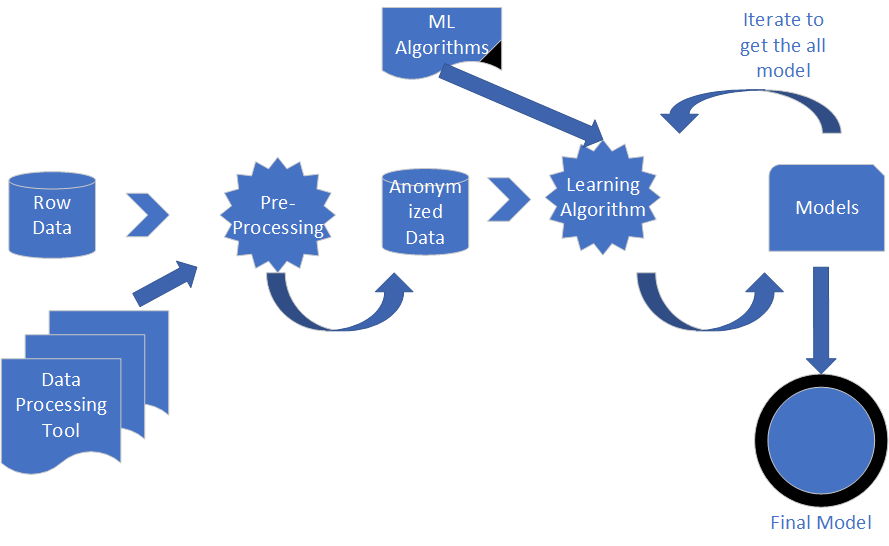
\includegraphics[scale=0.325]{media/framework/anonymization framwork.png}
    \caption{Anonymization Process}
    \label{fig:anonymization}
    \vspace{0mm}
\end{figure} 
\subsubsection{Evaluation Matrics}
\subsubsection{Results}
% It is possible to use a separate section for the Experimental Setup, which then focuses on all settings used in your experiments. It also possible to address the settings in a sub-section under Methodology. 




